% 2010 年四川卷文科第 15 题：二面角 α-l-β，AB⊂α，AB 与 l 成 30°。
% 来源 PDF：普通高考/2010/2010四川文.pdf，SHA-256 2e342add328217ef1fa0fc2a996f37d00cfc044a104397b29bdd75bedb1867fc。
% 原页：第 1 页（A3 三栏）第 3 栏上部，书页码 633。
% 重绘依据：l 为水平棱，α 向左上展开、β 向右下展开，AB 自 B 出发在 α 内斜上；
%   30° 标在 AB 与 l 之间但避开线段本身。
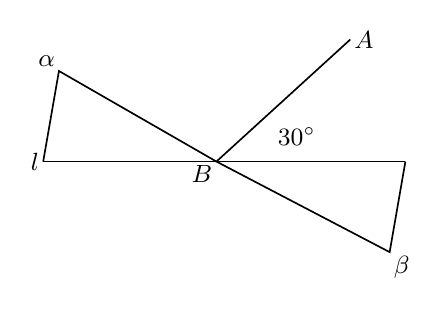
\begin{tikzpicture}[semithick, every node/.style={inner sep=1.2pt, font=\small}]
  \coordinate (B) at (0,0);
  \coordinate (l1) at (-2.2,0);
  \coordinate (l2) at (2.4,0);
  \coordinate (A) at (1.7,1.55);
  \coordinate (alpha1) at (-2.0,1.15);
  \coordinate (beta1) at (2.2,-1.15);
  \draw (l1) -- (l2);
  \draw (B) -- (A);
  \draw (l1) -- (alpha1) -- (B);
  \draw (l2) -- (beta1) -- (B);
  \node[left] at (l1) {$l$};
  \node[right] at (A) {$A$};
  \node[below left] at (B) {$B$};
  \node[above left] at (alpha1) {$\alpha$};
  \node[below right] at (beta1) {$\beta$};
  \node at (1.02,0.32) {$30^\circ$};
\end{tikzpicture}
